\chapter{Wstęp}

\section{Od kodu kreskowego do tagu radiowego}

Wraz z dużym postępem techniki oraz elektroniki w ostatnim dziesięcioleciu, niemal na każdym kroku spotykamy się z systemami automatycznej identyfikacji (ang. \emph{Auto ID}).  Umożliwiają one szybką , wygodną i bezbłędną identyfikacje produktów, sprzętu, ludzi a nawet zwierząt.  co usprawnia działanie systemów logistycznych. Technologie automatycznej identyfikacji znajdują coraz szersze zastosowanie we współczesnym świecie, głównie w obszarze przemysłu i transportu, przez handel, monitoring  po logistykę. Automatyczną identyfikację rozumiemy jako odczytywanie informacji o produkcie  w czasie rzeczywistym oraz następnie wprowadzenie tych danych do komputera w sposób w pełni zautomatyzowany czyli bez udziału człowieka.  Czytnik zbiera wszelkie możliwe informacje tym samym  zapewniając jednoznaczną, szybka i bezpieczną identyfikację obiektu.

Do najważniejszych systemów automatycznej identyfikacji zaliczamy:
\begin{itemize}\setlength{\itemsep}{0pt}
    \item kody kreskowe (ang. \emph{bar code}),
    \item karty elektroniczne  (ang. \emph{electronic cards}),ścieżki magnetyczne (ang. \emph{magnetic stripe}),
    \item systemy RFID (ang. \emph{Radio Frequency Identyfication}),
    \item systemy automatycznego rozpoznawania pisma ręcznego ICR (ang. \emph{Intelligent Charakter Recognition}) oraz rozpoznawanie znaków (druku)  OCR (ang. \emph{Optical Character Recognition}),
    \item systemy biometryczne:
	\begin{itemize}\setlength{\itemsep}{0pt}
		\item identyfikacja linii papilarnych,
		\item identyfikacja głosu,
		\item identyfikacja siatkówki oka,
		\item rozpoznawanie twarzy
	\end{itemize}
\end{itemize}

Intensywny i dynamiczny rozwój systemów \emph{Auto ID} miał swój początek w momencie wprowadzenia kodów kreskowych. Najpopularniejszego obecnie sposobu automatycznej identyfikacji obiektów.
Kod kreskowy inaczej określany jako kod paskowy (ang. \emph{bar code}) jest graficzną formą zapisu znaków, pod postacią ciemnych i jasnych pasków o zróżnicowanej szerokości, według przyjętej symboliki  (przyjętych reguł budowy danego kodu). Skanowanie kodu odbywa się z użyciem czytnika elektronicznego, który emituje cienką wiązkę światła.
Przesuwając się wzdłuż kodu wiązka lasera jest  pochłaniana przez ciemne paski kodu natomiast odbijana przez jasne fragmenty kodu i odbierana przez fotodiodę.
Siła sygnału, który powstaje w czytniku zależy od tego czy światło jest pochłaniane czy odbijane przez paski kodu, natomiast długość trwania sygnału zleży od grubości pasków. W rezultacie otrzymujemy jest ciąg sygnałów elektrycznych o różnej długości i natężeniu. Impulsy elektryczne tłumaczone są przez dekoder czytnika na cyfry, litery lub inne znaki, i przesyłane do komputera. 
Kody kreskowe są powszechnym i tanim sposób etykietowania produktów. Zaletą tego systemu jest powszechna unifikacja sposobu kodowania. Wadami  natomiast mała pojemność pamięci kodów kreskowych oraz częsty problem z odczytem danych (dane trzeba wprowadzać ręcznie). Duży problem w wielu sytuacjach stanowi również niewielka dopuszczalna odległość kodu od czytnika. 
Technologia kodów kreskowych jest obecnie najpowszechniejszą i najtańszą technologią znakowania produktów, jednak osiągnęła już swoje granice możliwości – w pewnych zastosowaniach jest już niewystarczająca.
Coraz większą popularność zyskuje technika radiowej identyfikacji – \emph{RFID}. System jest bardzo prosty dzięki temu zyskuje na popularności zarówno przy dużych i kosztownych projektach jak również  niewielkich przedsięwzięciach.

\newpage

\section{Struktura systemu \emph{RFID}}

RFID (ang.\emph {Radio Frequency  Identyfication}) to jedna z najszybciej rozwijających  się automatycznych technologii bezprzewodowej  identyfikacji radiowej. Jest to system tani, wszechstronny i niezawodny. Technologia \emph{RFID} wykorzystuje sygnał radiowy niskiej mocy do bezprzewodowej transmisji danych pomiędzy czytnikiem lub dekoderem  (ang.\emph{reader, interrogator}), a znacznikiem, inaczej zwanym transponderem lub identyfikatorem (ang. \emph{transponder, tag}). Dlatego też nie ma konieczności bezpośredniego kontaktu między etykietą, a czytnikiem.

\subsection{Budowa poszczególnych podzespołów systemu}

W skład typowego systemu \emph{RFID} wchodzą następujące podzespoły:

\begin{itemize}\setlength{\itemsep}{0pt}
	\item znacznik  (etykieta, transponder, identyfikator, tag, chip, metka) –zbudowany z układu elektronicznego lub microchipa z pamięcią, w którym dane są  kodowane i zapisywane w pamięci podręcznej oraz transmitowane za pomocą anteny nadawczo odbiorczej (często napylanej na warstwie izolatora). Cały układ identyfikatora przytwierdzony jest na nośnika np. papieru, plastiku. 

	Znaczniki \emph{RFID} mogą zawierać zarówno informacje zapisane w formie elektronicznej (pod postacią danych) jak również naniesiony tekst lub kod kreskowy. 

	Identyfikatory możemy sklasyfikować na dwa sposoby . W zależności od sposobu zasilania oraz od konfiguracji w jakiej występują.

	Pod względem zasilania transpondery dzielimy na: pasywne  (ang. \emph{passive}) (bez wewnętrznego zasilania) do zasilania  wykorzystują energie pola elektromagnetycznego, która wytwarzana jest przez czytnik oraz aktywne (ang. \emph{active}) (z własnym źródłem zasilania np. baterią) oraz półaktywne lub półpasywne (ang. \emph{semi-active, ang. semi-passive}) łączą cech zarówno transponderów aktywnych jak i pasywnych. Transpondery te wyposażone są w baterię zapewniającą zasilanie obwodom elektronicznym, natomiast nie posiadają nadajnika. Zasięg odczytu sięga 100 m, w dużym stopniu jednak zależy od czułości odbiornika w czytniku.  

	Znaczniki aktywne osiągają większą moc sygnału transmitowanego z identyfikatora, ponadto transmisja trwa krócej. Stosuje się je przede wszystkim do identyfikacji pojazdów. Najczęściej używane są znaczniki pasywne. Charakteryzują się brakiem własnego zasilania. Energię czerpią z fal radiowych celem odczytu i transmisji danych.  Konfiguracje w jakich może występować pamięć etykiety \emph{RFID} to: \emph{RO} (ang.\emph{read only}) - tylko odczyt – są programowane podczas produkcji i zawierają numer seryjny (mogą zawierać również inne dane , których nie można modyfikować), \emph{RW} (ang.\emph{read write}) - odczyt i zapis – dane mogą być wielokrotnie modyfikowane (pamięć może być podzielona na dwie części: część tylko do odczytu i część w której użytkownik może modyfikować zapisane dane) oraz \emph{WORM} (ang.\emph{write once read many}) -jednokrotny zapis i wielokrotny odczyt, część danych zapisana jest trwale, a część może być zmieniona przez użytkownika.
	
	\item czytnik  - zbudowany z mikrokomputera, który weryfikuje poprawność otrzymanych informacji, modułu transmisji radiowej czyli nadajnika i odbiornika  odpowiedzialnych za odczyt i zapis danych w identyfikatorze oraz antenę lub cewkę. Niektóre czytniki posiadają dodatkowo interfejs łączący z komputerem \emph{PC} (pozwalający na transmisję danych pomiędzy czytnikiem a komputerem).
	
	Oprogramowanie czytnika składa się z warstwy komunikacyjnej i użytkowej. Warstwa komunikacyjna odpowiedzialna jest za techniczną stronę transmisji danych, a warstwa użytkowa jest odpowiada za poprawne działanie aplikacji czyli wymianę, gromadzenia i przetwarzanie informacji. W zależności od budowy układ pracuje na komputerze i/lub na serwerze.Im większy czytnik tym większy jego zakres odczytu.
	
	Klasyfikacji czytników można dokonać według dwóch kryteriów. Pierwszy podział oparty jest na kryterium mobilności czytnika: stacjonarne (pracujące w trybie autonomicznym – cały czas sczytuje etykiety znajdujące się w jego zasięgu lub trybie interaktywnym –w tym trybie komunikacja odbywa się za pomocą aplikacji pracującej na serwerze lub aplikacji klienckiej), ruchome, przenośne.
	
	Drugi podział klasyfikuje czytniki na podstawie typu interfejsu komunikacyjnego:
	Szeregowe (porty RS-232 lub RS-485), sieciowe (z interfejsem sieciowym np. Ethernet).

\end{itemize}

Technologia \emph{RFID} w ostatnim dziesięcioleciu zyskała miano jednego z najbardziej obiecujących i najprężniej rozwijających się systemów identyfikacji na częstotliwości radiowej.  System \emph{RFID} pozwala na dużą automatyzację pracy zarówno podczas zapisu jak i odczytu danych. W przeciwieństwie do kodów kreskowych technologia ta nie wymaga bezpośredniej widoczności pomiędzy etykietą, a czytnikiem oraz daje możliwość czytania i przetwarzania wielu etykiet równocześnie.

\section{Organizacja systemu \emph{RFID}}

Zasada działania systemu opiera się na systemie komputerowym z bazą danych (w którym przechowywane  są wszystkie dane o ,,zametkowanym” produkcie)  oraz dwóch modułach identyfikacji radiowej: identyfikatorze i czytniku. Identyfikator – mały układ scalony z umieszczoną wewnątrz anteną w zależności od potrzeb i przeznaczenia zatopiony w plastiku, żywicy lub w formie etykiety samoprzylepnej na opakowaniu czy urządzeniu Każda etykieta posiada swój indywidualny niepowtarzalny numer identyfikacyjny \emph{ID}, który odnosi się do konkretnej bazy danych. W celu odczytania danych z tagu, nadajnik czytnika \emph{RFID} emituje pole elektromagnetyczne o częstotliwości rezonansowej układu odbiorczego. Antena dipolowa transpondera na  swoich końcach w skutek wywołanej różnicy  potencjałów indukuje prąd i magazynuje energię w kondensatorze.  Zgromadzona energia pobudza identyfikator do wysyłania odpowiedzi zawierającej kod znacznika. 
Czytnik wyposażony w antenę odbiorcza o dużej czułości, wykrywa, filtruje, demoduluję i dekoduje odebrane fale, tak aby odczytać odpowiedzi z transponderów.
Istnieje możliwość czytania i przetwarzania wielu etykiet (znajdujących się w zasięgu czytnika) równocześnie.Dane zapisane na etykiecie można odczytać w dowolnym momencie. 

Znaczniki, które nie  mają własnego zasilania (znaczniki pasywne), zasilane poprzez pole elekromagnetyczne magazynują energię w kondensatorze, która następnie zasila poszczególne obwody transpondera. Stosunkowo małe wymiary i niski koszt  produkcji transponderów pasywnych pozwala na masowe zastosowanie w wielu sektorach gospodarki. Natomiast transpondery aktywne, znajdując się w polu działania czytnika, pobierają energię ze swojej baterii, aby wysłać przechowywane dane, a co za tym idzie zapewniają większy zasięg nawet do kilkuset metrów, jednak są większe i znacznie droższe niż znaczniki pasywne.

\newpage

\section{Zakresy częstotliwości}

Systemy \emph{RFID} są jednym z wielu systemów radiowych, dlatego aby zapewnić bezkolizyjność pracy i zniwelować zakłócenia pomiędzy poszczególnymi systemami wprowadzono podział na zakresy częstotliwości.  Dozwolone dla systemów RFID przedziały częstotliwości zawarte są w pasmie radiowym ustandaryzowanym na całym świecie pod nazwą \emph{ISM} (ang. \emph{Industrial, Scientific, Miedical}). Jest to pasmo nielicencjonowane w zamyśle przeznaczone do zastosowań przemysłowych, badawczych i medycznych. Po za pasmem \emph{ISM} dostępne są dodatkowo niskie częstotliwości poniżej 135 kHZ.

Wyróżnić można kilka najpopularniejszych zakresów częstotliwości wykorzystywanych przez identyfikatory RFID:

\begin{itemize}\setlength{\itemsep}{0pt}
	\item pasmo niskich częstotliwości (ang. \emph {LF – Low Frequency}) – systemy \emph{RFID} działają zazwyczaj na częstotliwościach: 125 kHz i 134.2 kHz.
Transpondery \emph{LF} to zazwyczaj tagi pasywne, które odróżnią się od  transponderów pozostałych pasm częstotliwości małą wrażliwością na występowanie w pobliżu elementów metalowych, substancji płynnych oraz innych elementów wykonanych z dobrych przewodników. Dlatego świetnie sprawdzają się jako identyfikatory narzędzi, podzespołów maszyn, pojazdów czy metalowych kontenerów. Znalazły również zastosowanie w dziedzinie rolnictwa do znakowania zwierząt, leków oraz produktów spożywczych, gdyż pole niskich częstotliwości przenika przez tkanki ciała i płyny.
Wygląd i budowa transpondera \emph{LF} zależy ściśle od jego przeznaczenia. Transpondery używane jako immobilizery (czyli elektroniczne zabezpieczenia przed niepowołanym uruchomieniem pojazdu) zazwyczaj wbudowane są w kluczyk natomiast cewka anteny czytnika \emph{RFID} umieszczona współosiowo w stacyjce samochodu.
   
	\begin{figure}[h!]
	\centering
	    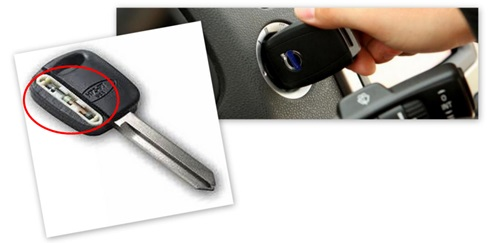
\includegraphics[width=9.32cm]{immobilizer.jpg}
	    \caption{Immobilizer}
	\end{figure}

	\newpage

	Zakres fal do 135 kHz znalazł również zastosowanie zarówno w systemach automatycznej identyfikacji jak i w znakowaniu zwierząt  zarówno hodowlanych jak i domowych.

	\begin{figure}[h!]
	\centering
	    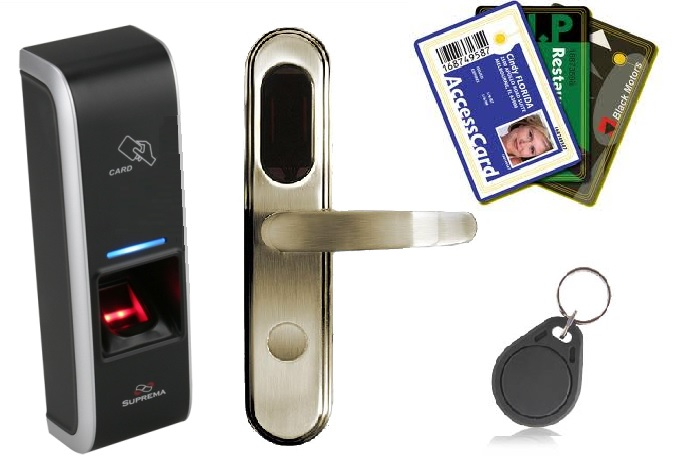
\includegraphics[width=7.27cm]{automatyczna_identyfikacja.jpg}
	    \caption{System automatycznej identyfikacji}
	\end{figure}
	
	\begin{figure}[h!]
	\centering
	    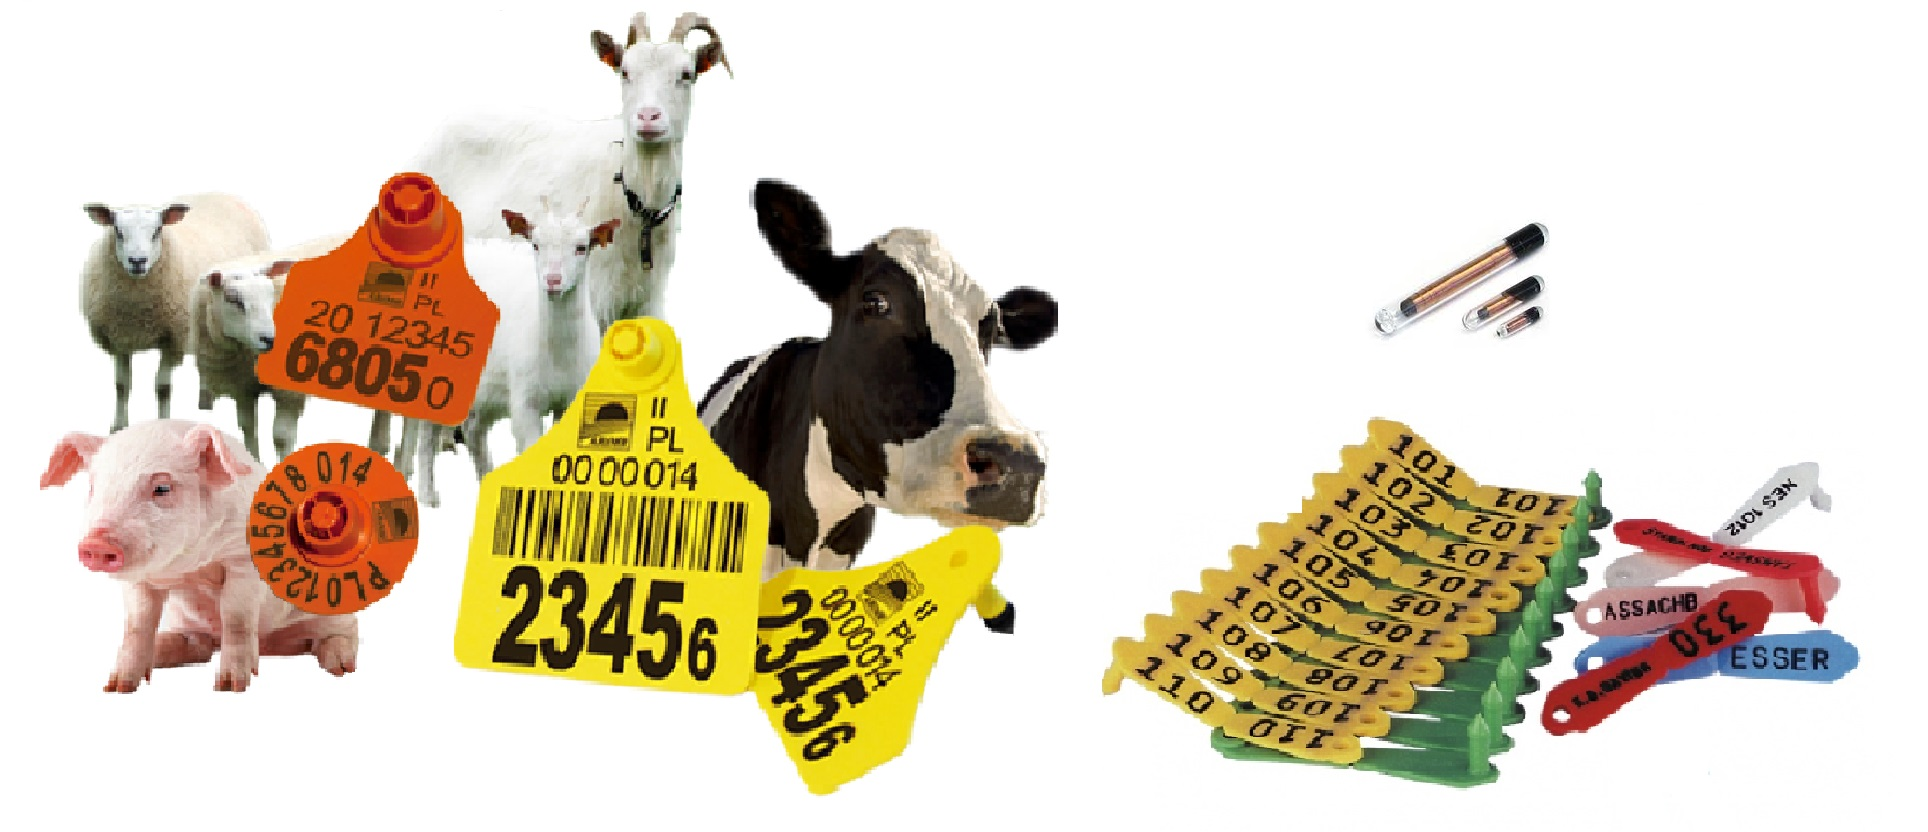
\includegraphics[width=14.34cm]{znakowanie_zwierzat.jpg}
	    \caption{Mikroczipy i kolczyki stosowane do znakowania zwierząt oraz kapsułki (biochipy) do wszczepiania pod skórę}
	\end{figure}
	
	Znaczniki pracujące w paśmie nie należącym do \emph{ISM} zbudowane są z ferrytowego rdzenia, na którym nawinięte są zwoje (około 100 zwojów) lub w postaci nadrukowanych zwojów na powierzchni materiału. Występują w formie plastikowych kart, krążków, biochipów, pastylek. Wadami tagów \emph{RFID} pracujących na częstotliwości LH jest: mała szybkość transmisji danych (1-2 kb/sek) - co znacznie ogranicza możliwą do zapisania odczytania ilość danych, niewielki zasięg – około 0.5 metra, podatność na zakłócenia przez urządzenia elektryczne  - co ogranicza zastosowanie w przemyśle. Problemem może być również limit jednoczesnego odczytu nie więcej niż 20 transponderów – ogranicza to pojemność systemu i maksymalną liczbę odczytów jaką może obsłużyć jeden czytnik. 

	\item pasmo wysokich częstotliwości (ang.\emph{HF – High Frequency}) – najczęściej wykorzystywane częstotliwości w tym pasmie to 6.78 MHz, 13.56 MHz, 27.125 MHz oraz 40.68 MHz. 
Transpondery \emph{HF} pracujące w zakresie 13.553 MHz – 13.657 MHz (pasmo \emph{ISM}) to zazwyczaj tagi pasywne. Identyfikatory pracujące na wysokich częstotliwościach wykazują większa wrażliwość na obecność w swoim otoczeniu metali i mniejszy wpływ na zakłócenia elektromagnetyczne pochodzące od  innych urządzeń niż tagi \emph{LF}. Pamięć tagów \emph{HF}  ma znacząco większa pojemność, a szybkość komunikacji sięga 20 kbit/s. Główną różnicą w procesie produkcji tagów \emph{HF} jest zastosowanie anten mniejszych rozmiarów. Antena transpondera \emph{HF} zbudowana jest zazwyczaj z 3-8 zwojów, nadrukowana jest za pomocą przewodzącego lakieru na podłoże i zaprasowana w etykiecie. Znaczniki możemy spotkać pod postacią samoprzylepnych etykiet (ang.\emph{smart label}), które programowane są w momencie drukowania etykiety. Zaletami transponderów \emph{HF} są: znacząco mniejsze koszty wykonania w porównaniu z identyfikatorami LH, co umożliwia ich zastosowanie na większą skalę, niewielka grubość identyfikatora nawet 0,1 mm, możliwy odczyt do 50 znaczników jednocześnie (dzięki wprowadzeniu mechanizmów antykolizyjnych) co pozwala zastosować je do automatycznej identyfikacji produktów i obiektów.  Warunkiem poprawnego odczytu wielu tagów jest zachowanie pomiędzy nimi, odległości co najmniej 2-3 centymetrów. 
	
	Zasięg w paśmie HF dochodzi do 1.5 metra, stanowi to zaletę jeśli chodzi np. o karty płatnicze z opcją płatności zbliżeniowej. Niewielki zasięg (dla kart z możliwością płatności zbliżeniowej dodatkowo ograniczony do około 2 cm) jest w tym przypadku konieczny ze względów bezpieczeństwa, aby dane z identyfikatora nie zostały odczytane przez osoby niepowołane. 

	\begin{figure}[h!]
	\centering
	    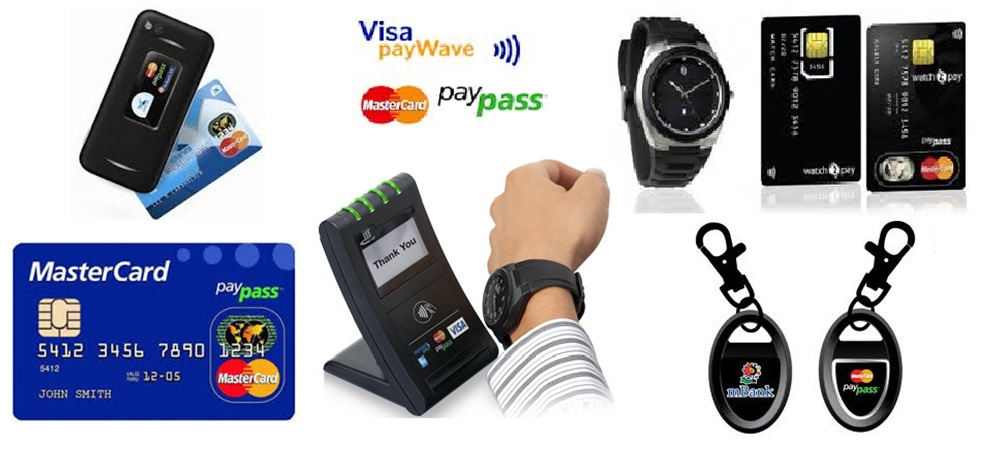
\includegraphics[width=16.56cm]{karty_platnicze.jpg}
	    \caption{Karty i breloki płatnicze}
	\end{figure}

	Systemy \emph{HF} są szeroko wykorzystywane gdyż posiadają możliwość wielokrotnego zapisu danych która jest niezbędna zarówno przy znakowaniu książek, dokumentów (paszportów, legitymacji studenckich, biletów komunikacji miejskiej, kart płatniczych) jak i bagażu na lotnisku czy odzieży w pralni.

	\begin{figure}[h!]
	\centering
	    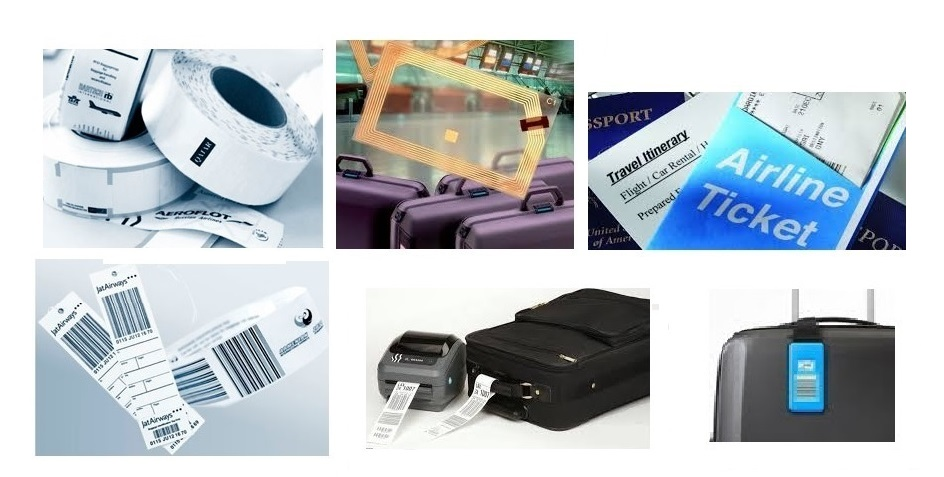
\includegraphics[width=15.51cm]{bagaz.jpg}
	    \caption{Znakowanie bagażu lotniczego}
	\end{figure}

	\begin{figure}[h!]
	\centering
	    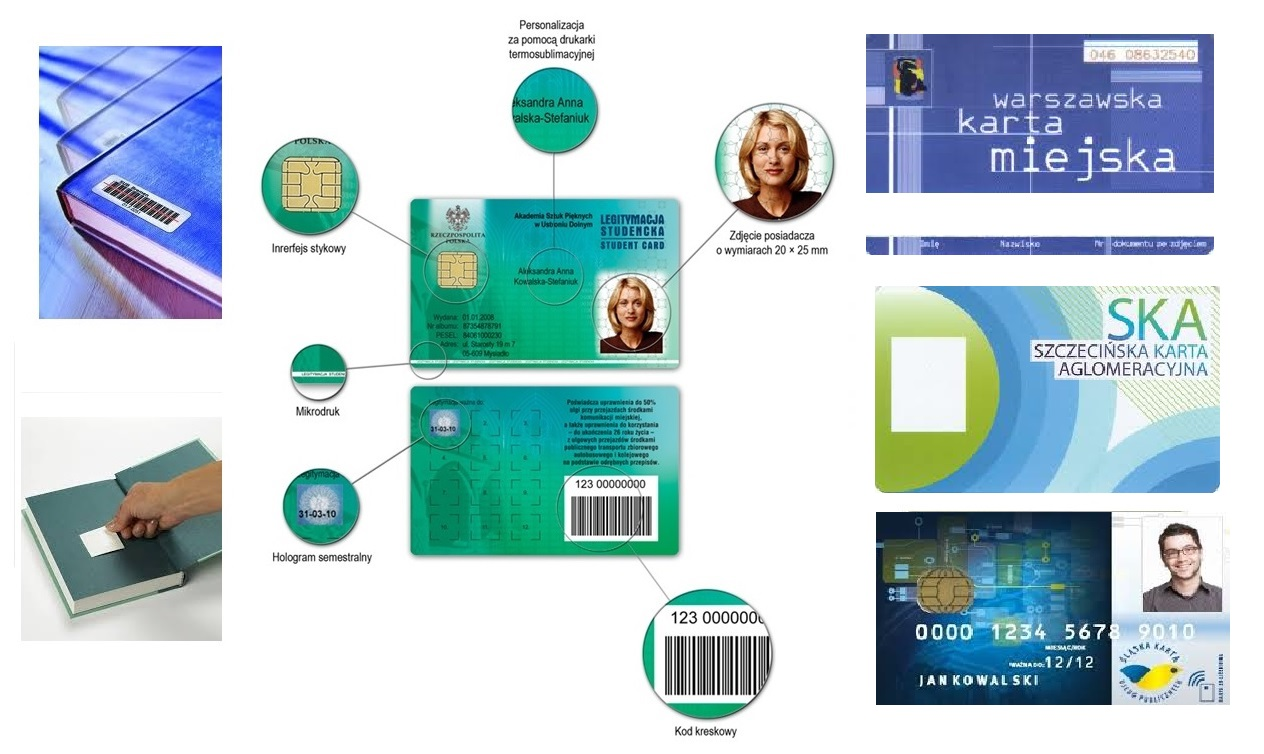
\includegraphics[width=16.82cm]{dokumenty.jpg}
	    \caption{Znakowanie książek, dokumentów, kart miejskich}
	\end{figure}
	
	Ciekawym wykorzystaniem systemów \emph{RFID}, które pracują w pasmie wysokich częstotliwości są systemy Eurobalise i Euroloop, stosowany w Europejskim Systemie Sterowania Pociągiem (ang. \emph{ETCS - European Train Control System}). Eurobalisa to urządzenie mocowane na torze pomiędzy szynami, które może komunikować się z przejeżdżającymi nad nim pociągami.


	\item pasmo ultra wysokich częstotliwości (ang. \emph{UHF – Ultra High Frequency}) – stosowane częstotliwości 433.92 MHz i 869.0 MHz, 915.0 MHz (poza Europą).
Występuje kilka zakresów częstotliwości \emph{UHF}: Europa 860-868 MHz, Ameryka Północna 902-928 MHz, Japonii  950 MHz-956MHz. W związku z różnicami w częstotliwościach pracy urządzeń, ustalono globalny standard.  W celu objęcia globalnego łańcucha dostaw stworzono identyfikatory i czytniki, która mogą pracować na całym świecie. Ważną zaletą technologii \emph{RFID} w pasmie \emph{UHF} jest największy zasięg dla identyfikatorów pasywnych spośród wszystkich pasm częstotliwości. Zaimplementowano lepsze protokoły antykolizyjne niż w systemach \emph{HF}. Wskutek tego zwiększyła się możliwość odczytu transponderów do 200 w jednym cyklu odczytu.  Zasięg odczytu sięga od 3 do 6 metrów – dlatego tagi \emph{UHF} chętnie stosowane są w magazynach.  Duża prędkość przesyłania danych od 40 do 120 kb/sek.  
Podobnie jak znaczniki \emph{HF} nie mogą być używane w pobliżu elementów metalowych, substancji płynnych i innych dobrych przewodników. 
Znaczniki \emph{UHF} ze względu na duży zasięg bardzo często stosowane są do śledzenia obiektów w logistyce. Wiele firm logistycznych, handlowych i spedycyjnych używa tylko i wyłącznie tagów \emph{UHF} ze względu na bardzo niski koszt produkcji, wynoszący kilkanaście groszy. 
Częstotliwość \emph{UHF} jest najbardziej rozpowszechnioną częstotliwością w logistyce i produkcji.

	\begin{figure}[h!]
	\centering
	    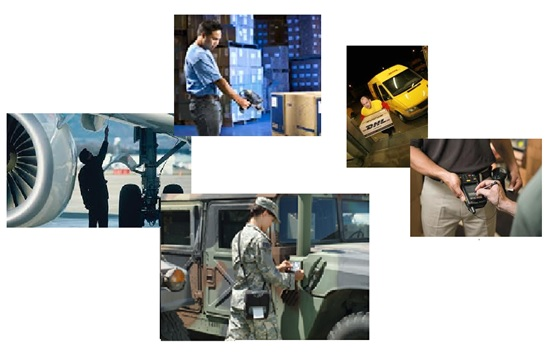
\includegraphics[width=14.37cm]{logistyka_transport_przemysl.jpg}
	    \caption{Przykłady zastosowań tagów UHF w sektorze logistyki, produkcji, transportu i handlu}
	\end{figure}

	\item pasmo mikrofalowe (ang. \emph{MW – Microwave}) – najpopularniejsze częstotliwości to 2.45 GHz, 5.8 GHZ i 24.125 GHz.  
Identyfikatory działające w tym paśmie są zazwyczaj aktywne lub pasywno-aktywne. Są stosunkowo mniejsze niż tagi pracujące na innych pasmach częstotliwości jednak droższe. Zasięg odczytu dochodzi do kilkuset metrów. Najistotniejszą zaletą tagów pracujących na częstotliwości mikrofal okazał się wysoki transfer danych, który  umożliwił sczytywanie informacji z obiektów poruszających się ponad 100 km/h, co nie jest możliwe w technologii tagów \emph{LH} i \emph{HF}.  To pozwoliło na wykorzystanie tego pasma do identyfikacji środków transportu komunikacji miejskiej, samochodów poruszających się  na autostradzie (automatyczne naliczanie opłaty za przejazd autostradą) , rejestracji przejeżdżających pociągów, czy statków.

	\begin{figure}[h!]
	\centering
	    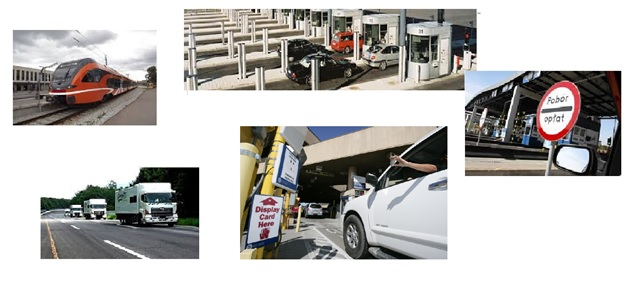
\includegraphics[width=16.61cm]{autostrady.jpg}
	    \caption{Naliczanie opłat za przejazd autostradą oraz identyfikacja środków komunikacji miejskiej}
	\end{figure}

	Znaczniki pracujące na częstotliwości 5.8 GHz montowane są w czujnikach przed drzwiami (w sklepach i marketach), w czujnikach ruchu jak również w systemach automatycznego spłukiwania toalet.
	Główną wada tagów \emph{MV} jest możliwość wystąpienia pomiędzy nimi a sieciami bezprzewodowymi (np. \emph{Wi-Fi}) interferencji. Możliwe zakłócenia odczytu w przypadku umieszczenia znaczników w pobliżu substancji płynnych lub metali.

\end{itemize}

System \emph{RFID} może pasować na wielu częstotliwościach, Nie ma możliwości ograniczenia systemu do jednego pasma pracy, gdyż tagi poszczególnych zakresów mają rózne własciwości, a co za tym idzie maja inne zastosowanie.

\newpage

\section{Przykłady zastosowania technologi \emph{RFID}}

Technologia \emph{RFID} znalazła zastosowanie w niżej wymienionych sektorach gospodarki: 

\begin{itemize}\setlength{\itemsep}{0pt}
	\item logistyka, transport i magazynowanie– potrzeba szybkiej identyfikacji i śledzenia poszczególnych elementów procesów logistycznych. Identyfikacja i rejestracja towarów w magazynie i na kolejnych etapach produkcji / dystrybucji.  Śledzenie przesyłek pocztowych / kurierskich, bagaży na lotnisku.  Tagi \emph{RFID} stopniowo wypierają etykiety logistyczne i kody kreskowe,

	\item sposoby płatności – karty płatnicze PayPass, systemy kart rabatowych w hipermarketach i na stacjach benzynowych, 

	\item elektroniczne bilety, karty wstępu – w komunikacji miejskiej, na imprezach masowych/sportowych, opłaty za przejazd autostradami, \emph{skipass} – karta identyfikacyjna narciarza umożliwiająca korzystanie z urządzeń w ośrodkach narciarskich, baseny lodowiska,

	\item organizacja pracy – kontrola dostępu do wyznaczonych miejsc poprzez umieszczanie znaczników \emph{RFID} w identyfikatorach (np. kartach, breloczkach). Pozwalają one na identyfikację właściciela, monitoring czasu pracy oraz system kontroli dostępu (inteligentne budynki),

	\item znakowanie zbiorów, odzieży – archiwa, muzea i biblioteki w których na książkach coraz częściej zamiast kodów kreskowych znajdują się tagi RFID, które ułatwiają identyfikacje jak również zabezpieczają przed kradzieżą. Znakowanie odzieży w celu rozpoznawania i sortowania m.in. pralniach jak i w sklepach również w celu ochrony przed kradzieżą jak i fałszerstwem produktów markowych,
 	
 	\item dokumenty, papiery wartościowe– tagi w postaci samoprzylepnych etykiet – zabezpieczenie podobne do hologramu. Śledzenie i zapisywanie historii obiegu oraz aktualnej lokalizacji ważnych dokumentów.  W paszportach stosowane w celu przechowywania danych osobowych oraz informacji na temat przekraczanych granic. Wymagane zabezpieczenie przed odczytem danych przez niepowołane osoby,
	
	\item przemysł – oznaczanie i  identyfikacja podzespołów, półproduktów oraz zapis poszczególnych stanów procesów produkcyjnych co pozwala na ich automatyzację. Śledzenie obiektów na liniach produkcyjnych, rejestracja danych. Identyfikacja cystern, wagonów pojemników w procesie produkcji
	
	\item dane eksploatacyjne maszyn – identyfikacja tonerów do drukarek – firmy zabezpieczają cartridge/tonery do drukarek, aby drukarki nie podejmowały pracy w momencie przekroczenia dopuszczalnej liczby wydrukowanych stron na jednym tonerze lub w przypadku gdy toner nie pochodzi do konkretnego producenta, 
	
	\item rolnictwo, znakowanie zwierząt hodowlanych, zagrożonych gatunków –oznaczanie zwierząt jest to jedno z najstarszych zastosowań technologii \emph{RFID}. W tym wypadku tagi \emph{RFID} występują w postaci charakterystycznych żółtych klipsów przymocowywane do uszu bydła i trzody chlewnej. Pozwalają na identyfikację zwierząt a co za tym idzie odczytanie m.in. miejsca ich chowu,
	
	\item sport – rejestrowanie czasów oraz ilości okrążenie w zawodach sportowych.  W przypadku masowych rozgrywek sportowych  nie możliwe byłoby odmierzanie czasu stoperem każdemu zawodnikowi,
	
	\item transpondery na oponach samochodowych – zawierają najczęściej numer identyfikacyjny, datę produkcji oraz stopień zużycia opony.

\end{itemize}

\newpage
\section{Wykorzystanie technologii \emph{RFID} w różnych sektorach gospodarki}

	\begin{figure}[h!]
	\centering
	    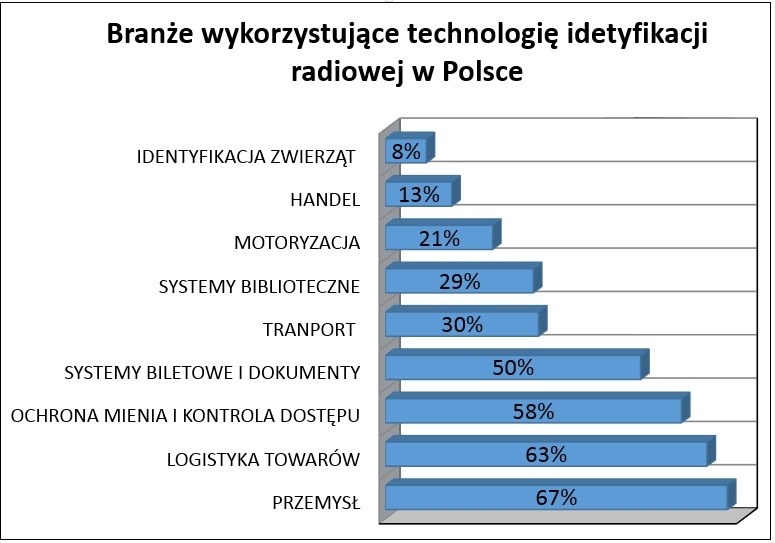
\includegraphics[width=16.2cm]{wykres_ver3.jpg}
	    \caption{Procentowy udział branż wykorzystujących technologię \emph{RFID}}
	\end{figure}


\section {Zalety i wady zastosowania systemu \emph{RFID}}

Zalety technologii \emph{RFID}:

\begin{itemize}\setlength{\itemsep}{0pt}
	\item nie jest wymagany optyczny kontakt zarówno przy zapisie jak i odczycie, czytnika z identyfikatorem, - dzięki temu operację ta można zautomatyzować i zrealizować szybciej,
	
	\item możliwość odczytu wielu identyfikatorów równocześnie,
	
	\item dużą  pojemność pamięci  - możliwość przechowywania większej ilości danych niż w przypadku kodów kreskowych

	\item możliwość aktualizacji / zmiany, wielokrotnego zapisywania i dopisywania danych  na etykiecie,

	\item identyfikatory mogą być wykorzystane wielokrotnie,

	\item duża prędkość transmisji danych,

	\item możliwość zapisywania danych również w trakcie ruchu obiektu,

	\item duże bezpieczeństwo danych -istnieje możliwość zastosowana różnych metod ochrony danych zapisanych na znaczniku, zabezpieczenie dostępu do pamięci, zabezpieczenie dostępu hasłem,  

	\item miniaturyzacja tagu  - najmniejszy wyprodukowany na świecie tag przez firmę Hitachi posiada wymiary 0,05 x 0,05 mm

	\item możliwość pracy w trudnych warunkach przemysłowych –  w miejscach gdzie występuje duże zapylenie, bardzo wysokie lub bardzo niskie ciśnienie, niska temperatura, agresywne chemikalia np. kopalnie, zakłady przemysłowe, chłodnie itp.

	\item możliwość integracji z istniejącymi systemami automatycznej identyfikacji (kody kreskowe),

	\item prędkość przemieszczania się ani ilość tagów nie wpływa na odczyt,

	\item możliwość wykorzystania tych samych identyfikatorów w całym łańcuchu dostaw.

\end{itemize}

Wady technologii \emph{RFID}:

\begin{itemize}\setlength{\itemsep}{0pt}

	\item brak jednolitego standardu dla protokołu RFID,
	
	\item możliwość zakłócenia przez odziaływanie elektromagnetyczne, wilgoć czy metale,
 	
 	\item większy koszt pojedynczego znacznika, w porównaniu z kodem paskowym, zwłaszcza w przypadku znaczników o większej funkcjonalności 

\end{itemize}






\chapter{Cel i zakres pracy}

Celem niniejszej pracy było zaprojektowanie i wykonanie anteny tekstylnej przewidzianej do pracy w paśmie \emph{ISM} (2.4 GHz). Zakres pracy nad projektem obejmował kilka etapów:

\begin{itemize}\setlength{\itemsep}{0pt}
	
	\item stworzenie modelu symulacyjnego badanej anteny,

	\item symulacje zaproponowanej struktury anteny,

	\item przeprowadzenie analizy numerycznej,

	\item wykonanie modelu i przeprowadzenie badań eksperymentalnych wybranych parametrów anteny.

\end{itemize}

W trakcie realizacji założeń projektu pracowałam wykorzystując środowisko \emph{CST Microwave Studio}.  W programie zasymulowałam zaprojektowaną antenę, przeanalizowałam otrzymane wyniki i przyjrzałam się wybranym parametrom

\chapter {Projekt anteny}

\section{Wstęp}







	